% !TEX root = ../main.tex

\section{Introdução} % (fold)
\label{sec:introdu_o}

O desenvolvimento de software perpassa inúmeras fases até que o mesmo seja concluído e entregue ao cliente, uma dessas fases, e provavelmente a mais importante é a fase em que devemos entender o problema do usuário, compreender exatamente o que o mesmo necessita e apresentá-lo uma solução. Nesta fase, negociações serão feitas, tanto sobre funcionalidades do sistema quanto custo do projeto, tempo para conclusão do mesmo e restrições de projeto.

O resultado desta fase é uma documentação robusta, principalmente ao utilizar metodologias tradicionais de desenvolvimento. Nesta documentação se encontram as funcionalidades do software, as características do mesmo e as restrições de projeto, podendo abranger todo o software ou apenas uma primeira etapa de desenvolvimento, como é feito em metodologias ágeis, estes ítens são conhecidos como requisitos.

Com esta documentação em mãos, os desenvolvedores podem começar o desenvolvimento do sistema, porém muitos problemas surgem tanto na construção da documentação quanto na utilização da mesma para o desenvolvimento do software. A gerência, organização, classificação e rastreabilidade dos requisitos geram inúmeros problemas, já que o conteúdo é muito extenso para ser organizado facilmente de forma adequada. A partir deste problema, surge a necessidade da utilização de ferramentas que auxiliem na organização, classificação e rastreabilidade dos requisitos.

\subsection{Propósito}

Ao analisar este documento, todos os \stakeholder~ deverão compreender todo o contexto de negócio, os objetivos e escopo do projeto, assim como, entender o problema que deverá ser resolvido, quais necessidades do cliente deverão ser analisadas e quais serão as funcionalidades do sistema, assim como todas as suas características.

\subsection{Escopo}

Este documento abrange todo o contexto do desenvolvimento de software voltado para a fase de requisitos, desde a elicitação à gerência de requisitos. Encontra-se neste documento, o problema de negócio do cliente, suas reais necessidades, as características das mesmas e todas as funcionalidades do sistema.

Dessa forma, a partir deste documento, pode-se obter conhecimento total sobre o projeto de desenvolvimento da ferramenta de gerência de requisitos, desde a metodologia utilizada para o desenvolvimento até a forma de implementação do sistema.
%Descreve brevemente o escopo deste documento de visão, incluindo a quais programas, projetos, aplicativos e processos de negócios o documento está associado. Inclui qualquer outra coisa que este documento afete ou influencie.

\subsection{Definições, acrônimos e abreviações}

\begin{itemize}
	\item \stakeholder:

		Todos as partes envolvidas no contexto do sistema, desde o cliente e seus funcionarios até a equipe de desenvolvimento do sistema. Todos os interessados na solução de software são considerados stakeholders do sistema.

	\item \textit{Requisitos}: 

		Engloba tudo que o software deve possuir para solucionar o problema em questão, desde funcionalidades do sistema até características que o software deve possuir.

	\item \textit{Requisitos Funcionais}:

		São chamados de requisitos funcionais todos aqueles que apresentam as funcionalidades do sistema. \cite{sommerville2003engenharia}.

	\item \textit{Requisitos não Funcionais}:

		São chamados requisitos não funcionais todos aqueles que apresentam as características do sistema, incluindo compatibilidade, o tempo de resposta ou qualquer outra exigência que não inclua funcionalidades. \cite{sommerville2003engenharia}.

	\item \textit{Engenharia de Requisitos}:

		Engenharia de Requisitos é um conceito que engloba todo um contexto de desenvolvimento de software que envolve elicitação de requisitos, negociação, verificação e validação, e documentação e gerência de requisitos para o desenvolvimento de um sistema computacional. O uso da palavra \textit{Engenharia} garante que técnicas sistematicas serão utilizadas para que os requisitos sejam completos, corretos e consistentes \cite{de2004analise}. 

	\item \textit{Fishbone}:

		Consiste em uma técnica utilizada para o reconhecimento do problema macro do cliente. A utilização desta técnica garante uma facilidade maior para entender o problema de negócio.

	\item \textit{Framework do problema}:

		Consiste em uma técnica para organizar e auxiliar o entendimento do problema, apresentar os stakeholders afetados pelo problema, o impacto que o problema gera para o cliente e uma possivel soluçao bem sucedida. A utilização do framework garante maior facilidade no entendimento do contexto do cliente.

	\item \textit{Framework de Necessidades}:

		Consiste em uma técnica para oganizar uma tabela identificando Necessidade, Problema, Solução atual e Solução Proposta. A utilização do framework de necessidade garante um melhor entendimento da necessidade do cliente.
 
	\item \textit{WorkShop}

		 Workshop é uma tecnica no qual os partipantes discutem um problema em comum onde são aplicadas tecnicas que ajudam em uma melhor identificação das necessidades do cliente e ajudam a melhorar o rendimento das reuniões.

	\item \textit{Brainstorming}

		 Brainstorming é uma tecnica que consiste em uma dinamica de grupo para recolher ideias a respeito de um determinado assunto e para a resolução de problemas.

	\item \textit{Casos de Uso}:

		 Caso de uso define uma sequência de ações que produz um resultado de valor observável. Os casos de uso fornecem estrutura para expressar requisitos funcionais no contexto dos processos de negócio e de sistema.

	\item \textit{Sprint}:

		Representa o espaço de tempo no qual deverão ser realizadas atividades previamente estabelecidas para a resolução de um problema. \cite{beck2000extreme}.

	\item \textit{Release}:

		São entregas de código funcional, as quais são feitas por etapa, entregando pequenas partes do software de tempos em tempos. \cite{beck2000extreme}.

	\item \textit{Product Owner (PO)}:

		É o responsável pela atividade de repassar o conhecimento de todo o contexto de negócio para a equipe de desenvolvimento. Muitas vezes, o PO pode ser o próprio cliente ou qualquer funcionário que tenha conhecimento do problema e faz o intermédio entre a equipe de desenvolvimento e o cliente. \cite{beck2000extreme}

	\item \textit{Product Backlog}:

		Representa a produção do trabalho executado durante o desenvolvimento.\cite{sanches2010aplicaccao}.

	\item \textit{Sprint Backlog}:

		Representa o trabalho a ser desenvolvido durante uma \textit{sprint} com o objetivo de criar um produto apresentável para a equipe. O \textit{backlog} da \textit{sprint} deve ser produzido de forma incremental.

\end{itemize}
% Define todos os termos, acrônimos e abreviações necessários para interpretar a visão corretamente. Essas informações podem ser fornecidas por referência ao glossário do projeto, que pode ser desenvolvido online no repositório do RM.

\subsection{Visão geral}

Basicamente, neste documento, encontra-se todo o registro do contexto de desenvolvimento da Ferramenta de Gerência de Requisitos. O mesmo é organizado de forma a buscar o melhor entendimento a partir de qualquer \textit{stakeholder} do projeto, desde leigos até funcionários da área.
%Descreve o conteúdo do documento de visão e explica como o documento é organizado.

%\subsection{Objetivos} % (fold)
%\label{sub:objetivos}
%\subsubsection{Objetivos Gerais}

%O objetivos gerais deste projeto é a fase de requisitos e o início da implementação de uma ferramenta de gerência de requisitos \opensource{} que auxilie o usuário durante todo o processo de requisitos, desde a escolha da metodologia utilizada ao controle da rastreabilidade dos requisitos.

%\subsubsection{Objetivos Específicos}

%Objetivos especificos são pequenos marcos que serão realizados durante o projeto, são eles:

%\begin{itemize}
%	\item Entender e registrar os problemas da \er.
%	\item Entender e registrar as necessidades da \er.
%	\item Entender as caractrísticas da \er.
%	\item Definir requisitos funcionais para o desenvolvimento da ferramenta.
%	\item Definir requisitos não-funcionais para o desenvolvimento da ferramenta.
%	\item Definir casos de uso do desenvolvimento da ferramenta.
%	\item Definir escopo da ferramenta.
%\end{itemize}

%\subsection{Justificativas} % (fold)
%\label{sub:justificativas}

%Inúmeras ferramentas já foram criadas para esta finalidade, contudo as ferramentas gratuitas não possuem a qualidade necessária para desenvolvimento de grandes e críticos sistemas. A partir daí, surge a necessidade da criação de uma nova ferramenta \opensource{} com qualidade suficiente para suprir as necessidades de todos os desenvolvedores de software do mundo.

%Outra vantagem de uma ferramenta \opensource{} é a possibilidade de qualquer interessado em manter a ferramenta estar permitido a fazer o mesmo, o que facilita uma futura evolução do projeto, mantendo ele sempre capaz de se manter reais as necessidades do usuário. 
% section introdu_o (end)

\section{Processo de Engenharia de Requisitos}
\label{sec:processo}
% !TEX root = ../main.tex

Inicialmente, foi necessário entender o problema do qual seria tratado, traçar características e definir uma visão com o cliente para impedir problemas futuros, como, por exemplo, problemas de comunicação causados por ambiguidade, estas informações estão esclarecidas no Documento de Visão, presente na Sessão \ref{sec:document_de_visao} deste documento.

Após a definição do Problema iniciou-se a parte de elicitação de requisitos, tanto funcionais como não funcionais, a modelagem desta está representada na Figura \ref{img:modelagem1}.

\begin{figure}[H]
	\centering
	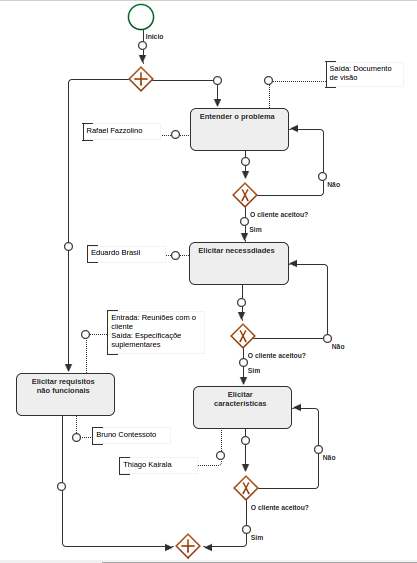
\includegraphics[width=0.8\textwidth]{imgModelagem/modelagem1}
	\caption{Modelagem Parte 1}
	\label{img:modelagem1}
\end{figure}


Após a definição dos casos de uso do projeto, deve-se definir as prioridades, criação dos \textit{roadmaps}, assim como detalhamento dos casos de uso e implementação das funcionalidades com maior prioridade do projeto, porém, durante o andamento, já estavam definidos os casos de uso que seriam implementados na primeira entrega, então foi feito em paralelo o plano de iteração e o primeiro \textit{roadmap}. A modelagem do mesmo esta presente na Figura \ref{img:modelagem2}.

O detalhamento dos casos de uso está presente na Sessão \ref{sec:documento_de_caso_de_uso} deste documento, assim como os \textit{roadmaps} se encontram na Sessão \ref{sec:road_map}.

\begin{figure}[H]
	\centering
	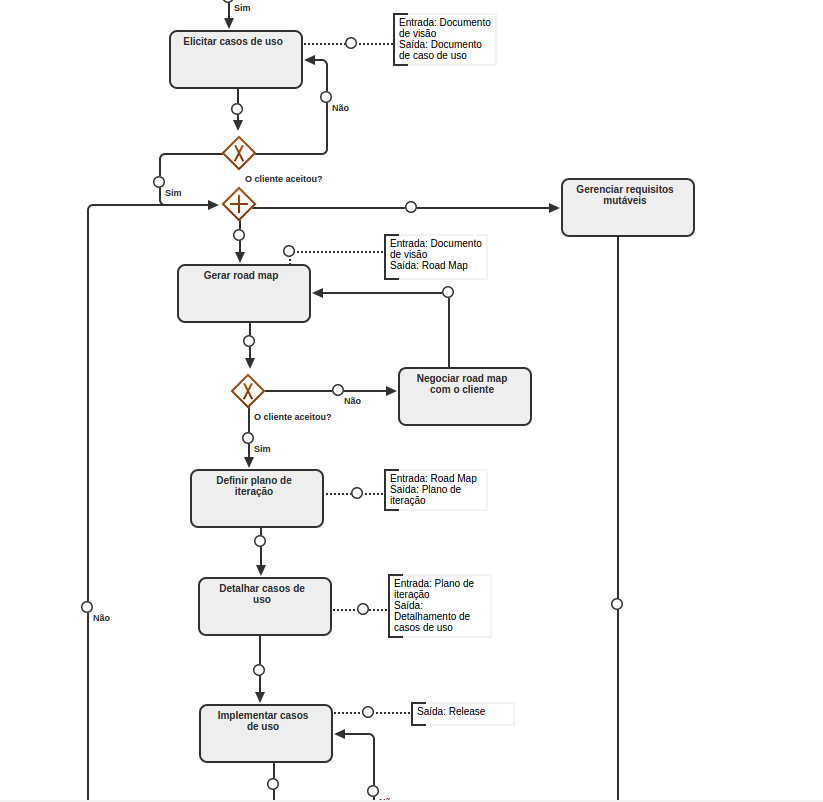
\includegraphics[width=1\textwidth]{imgModelagem/modelagem2}
	\caption{Modelagem Parte 2}
	\label{img:modelagem2}
\end{figure}

Após a implementação dos casos de uso da iteração, caso o cliente aceite, segue-se para a próxima iteração ou final do projeto, dependendo se existe ou não outros casos de uso a serem implementados, caso haja, o processo volta para as atividades de gerar o \textit{road map}  e gerenciar requisitos mutáveis presentes na Figura \ref{img:modelagem2}, assim como mostra a Figura \ref{img:modelagem3}.

\begin{figure}[H]
	\centering
	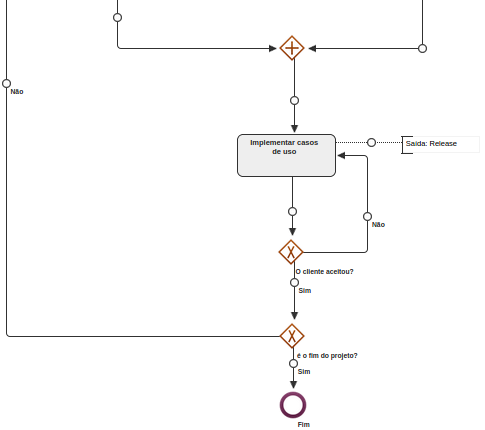
\includegraphics[width=1\textwidth]{imgModelagem/modelagem3}
	\caption{Modelagem Parte 3}
	\label{img:modelagem3}
\end{figure}


\section{Documento de visão}
\label{sec:document_de_visao}
% !TEX root = ../main.tex

O documento de visão tem como objetivo definir uma visão geral do projeto, apresentar os problemas, os requisitos funcionais, não funcionanis, atores, entre outras informações que serão definidos com o cliente a fim de garantir que a equipe de desenvolvimento e o cliente estejam na maior sincronia possível \cite{IBM:2014:Online}.

%-----------------------------------------------------------------------------------------------------------
\subsection{Posicionando}
\subsubsection{Oportunidade de Negócios}

Atualmente, as ferramentas no mercado possuem limitações, como de qualidade, falta de flexibilidade na gerência, ou até mesmo o fechamento do código, que pode ser considerado uma limitação devida a redução de mão de obra para manutenção e evolução.

\subsubsection{Instrução do Problema}

A \er{} possui diversas \textit{rotas} possíveis para se seguir, como, por exemplo a rota ágil, tradicional ou até mesmo uma mistura das duas.

Infelizmente, cada ferramenta de gerência de requisitos é voltada para uma dessas possibilidades, tornando díficil a tarefa voltada para outras, gerando assim nos engenheiros de requisitos a necessidade de aprender a utilizar diversas ferramentas para poder organizar projetos com \textit{rotas} diferentes.

A utilização de apenas uma ferramenta que abrangesse as duas metodologias e ainda uma mistura das duas resolveria todo problema de gerência de requisitos em projetos que não se adequam a uma metodologia específica perfeitamente.

\subsubsection{Instrução de Posição do Produto}

Para os engenheiros de \er, a \nomeferramenta~ representará um avanço nas atividades de gerenciamento, pois os mesmos apenas precisarão aprender as funcionalidades de uma ferramenta, simplificando a mudança entre projetos que tomam rotas distintas.

%-----------------------------------------------------------------------------------------------------------
\subsection{Matriz de rastreabilidade de requisitos}

A matriz de rastreabilidade resume o modo como serão organizados os requisitos do sistema, e a escolhida para o projeto esta ilustrada na figura \ref{img:rastreabilidade}.

\begin{figure}[H]
	\centering
	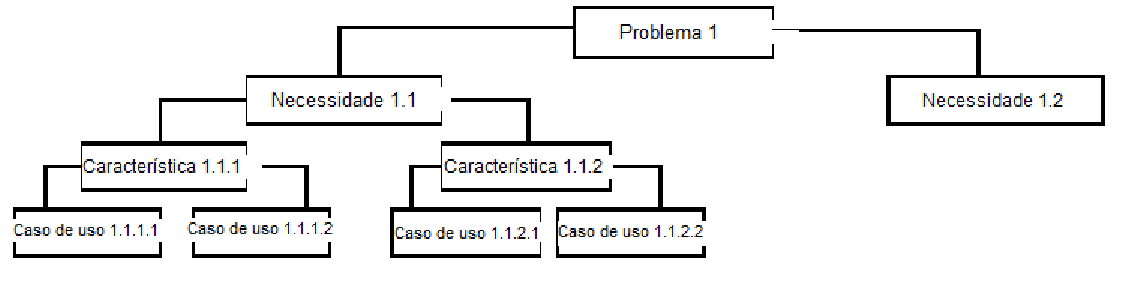
\includegraphics[width=0.8\textwidth]{imgModelagem/diagrama}
	\caption{Matriz de rastreabilidade}
	\label{img:rastreabilidade}
\end{figure}

%-----------------------------------------------------------------------------------------------------------
\subsection{Descrições da Parte Interessada e do Usuário}

Nesta sessão serão identificados e detalhados os interessados e usuários da \nomeferramenta{}.

\subsubsection{Resumo da Parte Interessada e do Usuário}

Para melhor entendimento das características e responsabilidades dos interessados, utilizou-se uma tabela que apresenta todos os interessados no sistema, suas descrições, responsabilidades e os critérios de sucesso de suas funções na equipe, ilustrada na tabela \ref{tab:parteInteressada}. Com esta tabela, pode-se obter o entendimento necessário sobre os interessados e o quão importante eles são para o sucesso do sistema.

\begin{table}[htbp]
\centering
\begin{tabular}{|p{2cm}|p{5cm}|p{4cm}|p{4cm}|}
\hline
%-------------------------------------------------------
\textbf{Interessado} &
\textbf{Descrição} &
\textbf{Responsabilidade} &
\textbf{Critérios de Sucesso}
\\ \hline

%-------------------------------------------------------
Analista de Requisitos &
Membro da equipe de desenvolvimento com facilidade em comunicação, psicologia, sociologia, filosofia e mais áreas que possam facilitar a relação com o cliente. Seu conhecimento na área pode ser, dependendo da organização, baixo. &
Pessoa responsável por realizar a elicitação dos requisitos junto ao usuário. Deve elicitar os requisitos de forma adequada à garantir sucesso no desenvolvimento do \sw. &
Requisitos corretamente elicitados e prontos para serem documentados. 
\\ \hline
%-------------------------------------------------------
Gerente de Requisitos &
Conhecedor de todo o processo de desenvolvimento e com contato frequente com o cliente. Seu conhecimento deve ser alto. &
Pessoa responsável por administrar os requisitos durante todo processo de desenvolvimento de \sw, garantindo o mínimo esforço em casos de mudança de requisitos. &
Requisitos bem administrados para, no caso de mudanças nos requisitos, existir o menor impacto possível na equipe de desenvolvimento.
\\ \hline
%--------------------------------------------------------
Programador &
Pessoa com capacidade em linguagens e lógica de programação &
Implementar o sistema utilizando as técnologias definidas &
Implementação do sistema de acordo com os requisitos levantados e cadastrados na ferramenta
\\ \hline

\end{tabular}
\label{}
\caption{Parte Interessada}
\label{tab:parteInteressada}
\end{table}

\subsubsection{Principais Problemas e Necessidades da Parte Interessada}

O problema a ser resolvido pela \nomeferramenta~ deve estar bastante claro entre todos os \stakeholder, para que o desenvolvimento passe pela menor quantidade possível de dificuldades quanto ao entendimento de onde focar esforços para desenvolver a solução.

Para o mapeamento do problema principal e suas causas, foi utilizada a técnica do \textit{Diagrama de Ishikawa}, que se contra na figura \ref{img:fishbone}.

%-------------------------------------FISHBONE AQUI----------------------------------------
\begin{figure}[H]
	\centering
	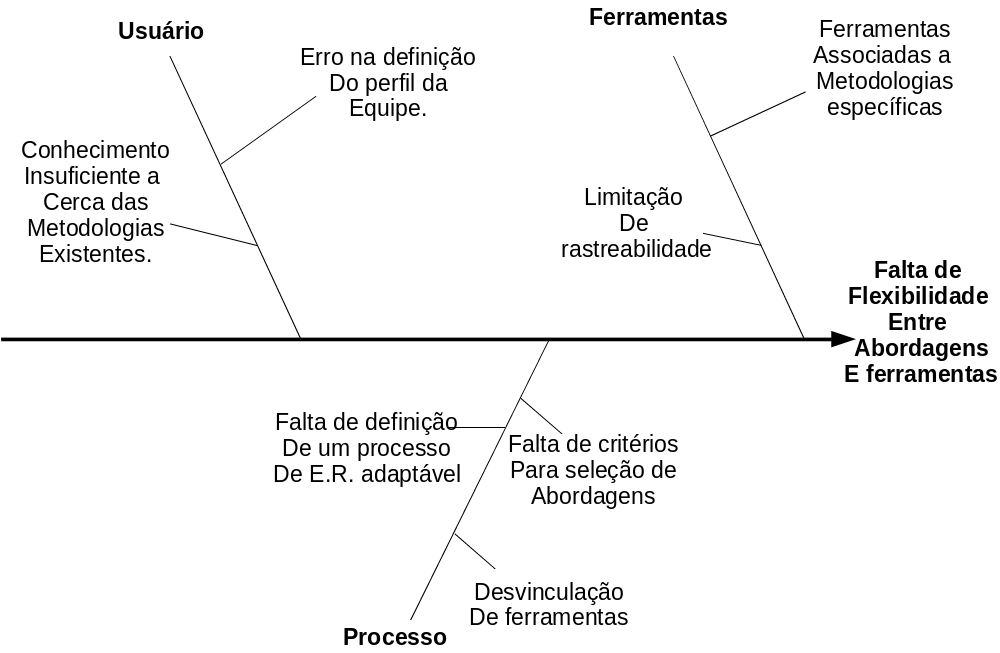
\includegraphics[width=0.8\textwidth]{imgModelagem/fishbone}
	\caption{Diagrama de Ishikawa}
	\label{img:fishbone}
\end{figure}
%-------------------------------------FISHBONE AQUI----------------------------------------


%-------------------------------------FRAMEWORK DE Problema-----------------------------------
Para melhor entendimento do problema, utilizamos a técnica de \textit{Framework de problema}, que consiste em criar uma tabela apresentando o problema, os afetados, o impacto e qual seria uma solução bem sucedida, o Framework esta retratado na tabela \ref{tab:frameworkproblema}.

\begin{table}[htbp]
\centering
\begin{tabular}{|p{3cm}|p{10cm}|p{2.5cm}|}
%----------------------------------------------
\hline
\textbf{O Problema:} &
Falta de flexibilidade entre Abordagens e Ferramentas. 
\\ \hline
%----------------------------------------------
\textbf{Afeta:} &
Todos os desenvolvedores de \sw~que necessitam de uma flexibilidade maior na gerência de requisitos.
\\ \hline
%----------------------------------------------
\textbf{Cujo impacto é:} &
Processo de requisitos mal gerenciados, aumentando a possibilidade de erros durante o desenvolvimento.
\\ \hline
%----------------------------------------------
\textbf{Uma solução bem sucedida seria:} &
Utilização de uma ferramenta que faça gerência de requisitos de forma flexivel, podendo utilizá-la em qualquer metodologia.
\\ \hline
%----------------------------------------------
\end{tabular}
\caption{Framework de Problema}
\label{tab:frameworkproblema}
\end{table}

%-----------------------------------------FRAMEWORK DE NECESSIDADES----------------------------------------
Após o entendimento do problema, vê-se necessária a documentação das necessidades do cliente. Utilizou-se de uma técnica chamada \textit{framework de necessidades} na qual são apresentados todos os problemas, as necessidades, a solução atual e a solução proposta. Dessa forma, pode-se obter um entendimento mais organizado dos problemas e necessidades do cliente, de acordo com o retradado na tabela \ref{tab:frameworknecessidade}.

\begin{table}[H]
\centering
\begin{tabular}{|p{5cm}|p{3cm}|p{3cm}|p{5cm}|}

%-------------------------------------------------------------
\hline
\textbf{Necessidade} &
\textbf{Problema} &
\textbf{Solução Atual} &
\textbf{Solução Proposta}
\\ \hline
%-------------------------------------------------------------
Utilização de ferramentas que se adequem as metodologias. &
Ferramentas associadas a metodologias específicas. &
Equipe utiliza mais de uma ferramenta para abranger as abordagens utilizadas. &
Criação de uma ferramenta que seja flexível para qualquer metodologia, abrangendo todas as agordagens e até a mesclagem das mesmas.
\\ \hline
%-------------------------------------------------------------
Apoio a utilização de uma rastreabilidade organizada e eficiente em qualquer abordagem. &
Limitação de ratreabilidade. &
A equipe precisa criar sua rastreabilidade sem o apoio de uma ferramenta flexível. &
Criação de uma ferramenta que gere a rastreabilidade dos requisitos de forma organizada e eficiente para qualquer abordagem.
\\ \hline
%-------------------------------------------------------------
Obter critérios fixos que redirecionem o projeto para a abordagem mais adequada. &
Falta de critérios para seleção de abordagens. &
Equipe precisa estudar as características do projeto e decidir qual a abordagem mais adequada. &
Criação de uma ferramenta que recolha as características do projeto e apresente a abordagem mais adequada.
\\ \hline
%-------------------------------------------------------------
Utilização de apenas uma ferramenta de gerência de requisitos durante o projeto. &
Desvinculação de Ferramentas. &
Equipe utiliza mais de uma ferramenta. &
Criação de uma ferramenta que garanta as funcionalidades de todas as ferramentas baseadas em distintas abordagens. 
\\ \hline
%-------------------------------------------------------------
Obter um processo de \textit{E.R.} adaptável a qualquer abordagem. &
Falta de definição de um processo de \textit{E.R.} adaptável. &
Utilização de um processo inflexível e voltado apenas para uma abordagem. &
Criação de uma ferramenta que gerencie processos flexíveis.
\\ \hline
%-------------------------------------------------------------
Obter o perfil da equipe de forma adequada. &
Erro na definição do perfil da equipe. &
Equipe precisa definir o próprio perfil. &
Criação de uma ferramenta que receba \textit{inputs} das características da equipe e apresente o perfil da equipe de forma correta.
%-------------------------------------------------------------
\\ \hline
Utilização da metodologia mais adequada para as características do projeto.&
Conhecimento insuficiente a cerca das metodologias existentes. &
Equipe precisa estudar todas as metodologias para escolher a mais adequada. &
Criação de uma ferramenta que apresente a metodologia mais adequada para o projeto.
\\ \hline
%-------------------------------------------------------------
\end{tabular}
\caption{Framework de Necessidades}
\label{tab:frameworknecessidade}
\end{table}

%-----------------------------------------------------------------------------------------------------------
\subsection{Visão Geral do Produto}
	
Nesta seção, pode-se ter um entendimento geral de como será o produto final, quais serão suas características, como serão suas funcionalidades e etc.

\subsubsection{Perspectiva do Produto}
	
O produto se encontrará em um contexto onde existem inúmeras ferramentas com o mesmo propósito, porém, as ferramentas existentes são inflexíveis quando se trata da abordagem que será seguida durante o desenvolvimento de \sw. Esta falha será corrigida na \nomeferramenta, que irá propor uma metodologia para cada projeto em particular de acordo com suas características.

A ferramenta pode ser autocontida, não necessitando do apoio de nenhum outro sistema, porém a utilização de ferramentas de modelagem de processos é bastante indicada para que a máxima organização do projeto seja alcançada.

\subsubsection{Resumo das Capacidades}
	
O grande diferencial da \nomeferramenta~ será a flexibilização na abordagem que será seguida durante o gerenciamento de projetos de \sw. O sistema deverá indicar a melhor abordagem a ser seguida pela equipe de desenvolvimento, garantindo a otimização do processo de desenvolvimento.

A ferramenta será capaz de disponibilizar a opção de modificar a abordagem indicada pela ferramenta, para que a equipe de desenvolvimento possa escolher a abordagem na qual os mesmos se sentem mais a vontade.

%-----------------------------------------------------------------------------------------------------------
\subsection{Recursos do Produto}
\label{subsub:recursos_produto}

Os recursos do produto são as funcionalidades do sistema com uma pequena descrição, o que futuramente será transformado em casos de uso, estes recursos estão organizados de acordo com a rastreabilidade proposta na figura \ref{img:rastreabilidade}, e serão detalhados no documento de casos de uso, presente na sessão \ref{sec:documento_de_caso_de_uso} deste documento, e estão listados a seguir.

\subsubsection{Problema 1 - Falta de flexibilidade entre abordagens e ferramentas}

O problem 1, gera algumas necessidades, que serão colocadas a seguir.

\paragraph{Necessidade 1.1 - Utilização de ferramentas que se adequem as metodologias\\}

	\begin{itemize}

	\item Caso de uso 1.1.1 - Manter Problema
	\item Caso de uso 1.1.2 - Manter Necessidades
	\item Caso de uso 1.1.3 - Manter Características
	\item Caso de uso 1.1.4 - Manter Casos de Uso
	\item Caso de uso 1.1.5 - Manter Temas de Investimento
	\item Caso de uso 1.1.6 - Manter Épicos
	\item Caso de uso 1.1.7 - Manter Features
	\item Caso de uso 1.1.8 - Manter Histórias de Usuário

	\end{itemize}

\paragraph{Necessidade 1.2 - Apoio a utilização de uma rastreabilidade organizada e eficiente em qualquer abordagem\\}

	\begin{itemize}
	\item Caso de uso 1.2.1 - Manter Atributos
	\item Caso de uso 1.2.2 - Manter Rastreabilidade de Requisitos
	\end{itemize}

\paragraph{Necessidade 1.3 - Obter critérios fixos que direcionem o projeto para abordagem mais adequada\\}

\paragraph{Necessidade 1.4 - Utilização de apenas uma ferramenta de gerência de requisitos em diferentes projetos\\}

\paragraph{Necessidade 1.5 - Obter um processo de \er~ adaptável a qualquer abordagem\\}

\paragraph{Necessidade 1.6 - Obter o perfil da equipe de forma adequada\\}

\paragraph{Necessidade 1.7 - Utilização da metodologia mais adequada para as características do projeto\\}

	\begin{itemize}
	\item Caso de Uso 1.7.1 - Definir Metodologia
	\item Caso de uso 1.7.2 - Definir ``hibridez'' do projeto
	\end{itemize}

 Estes são os casos de uso que nao se encaixam em nenhuma necessidade, alem de terem necessidades que não possuem casos de uso e necessidade duplicadas.

\begin{enumerate}

	\item Gerar \textit{Diagrama de Ishikawa}
	\item Manter Atores do Projeto
	\item Gerar Diagramas de Casos de Uso
	\item Manter \textit{Roadmaps}
	\item Gerar plano de iteração
	
	\item Controlar histórico de versão
\end{enumerate}
%-----------------------------------------------------------------------------------------------------------
\subsection{Restrições}
\subsubsection{Restrição Técnica}

A ferramenta poderá ser executada pelos navegadores Google Chrome versão 37.0.2062.120 ou superior Firefox versão 33.0 ou superior, não sendo possível sua utilização no Internet Explorer ou Safari.

%Observe todas as restrições de design, restrições externas, como requisitos operacionais ou regulamentares) ou outras dependências.

%-----------------------------------------------------------------------------------------------------------
\subsection{Faixas de Qualidade}
%Defina as faixas de qualidade para desempenho, robustez, tolerância a falhas, usabilidade e características similares que o conjunto de recursos não descreve.

%-----------------------------------------------------------------------------------------------------------

\subsection{Atributos do Recurso}

Atributos de recursos são basicamente descrições dos requisitos em alguma área em específico. Durante o projeto foram utilizados os atributos de arquitetura, prioridade e status.

\subsubsection{Atributos de Arquitetura\\}

Atributos de arquitetura são atributos que definem a complexidade arquitetural de se implementar algum requisito, por exemplo, se haverá necessidade de alterar arquitetura do software, e estão retratados na tabela \ref{tab:atributo_arquitetura}

\begin{table}[H]
\begin{tabular}{|p{4cm}|p{11cm}|}
%-------------------------------------------
\hline
\textbf{Atributo} &
\textbf{Descrição}
\\ \hline

%-------------------------------------------
\textbf{Grande} &
Para implementar o requisito, a arquitetura sofrerá uma grande alteração
\\ \hline

%-------------------------------------------
\textbf{Média} &
A arquitetura terá uma alteração consideravel na implementação do requisito
\\ \hline

%-------------------------------------------
\textbf{Baixa} &
A arquitetura terá uma pequena alteração para sustentar o requisito
\\ \hline

%-------------------------------------------
\textbf{Nenhuma} &
O requisito não terá impacto nenhum na arquitetura do projeto
\\ \hline
\end{tabular}
\caption{Atributo de Arquitetura}
\label{tab:atributo_arquitetura}
\end{table}

\subsubsection{Atributo de Prioridade\\}

Atributos de prioridade são atributos que definem o quão importante um requisito é para o cliente, definindo se ele deve ser implementado o mais rápido possível ou se pode ter sua implementação adiada, estão retratados na tabela \ref{tab:atributo_prioridade}.

\begin{table}[H]
\begin{tabular}{|p{4cm}|p{11cm}|}

\hline
\textbf{Atributo} &
\textbf{Descrição}
\\ \hline

%-----------------------------------------
\textbf{Alta prioridade} &
Os requisitos marcados com este atributo são requisitos que possuem um grande interesse do cliente
\\ \hline

%-----------------------------------------
\textbf{Média prioridade} &
Os requisitos marcados por este atributo são requisitos que o cliente possui um grande interesse, porém não existe necessidade de implementá-lo rapidamente.
\\ \hline

%----------------------------------------
\textbf{Baixa prioridade} &
Os requisitos marcados por este atributo são requisitos que o cliente deseja, porém não são essenciais para o funcionamento da solução.
\\ \hline

\end{tabular}
\caption{Atributo de prioridade}
\label{tab:atributo_prioridade}
\end{table}

\subsubsection{Atributos de Status\\}

Atributos de status são atributos que indicam em que fase um requisito está, de acordo com a tabela a seguir, e estão retrados na tabela \ref{tab:atributo_status}

\begin{table}[h]
\begin{tabular}{|p{4cm}|p{11cm}|}

\hline
\textbf{Atributo} &
\textbf{Descrição}
\\ \hline

%-------------------------------
\textbf{Aceito} &
Requisito devidamente implementado e aceito pelo cliente
\\ \hline

%-------------------------------
\textbf{Implementado} &
Requisito implementado porém esperando aceitação
\\ \hline

%-------------------------------
\textbf{Detalhado} &
Requisito detalhado, esperando por implementação
\\ \hline

%------------------------------
\textbf{Elicitação aceita} &
Requisito elicitado e aceito pelo cliente porém sem detalhamento
\\ \hline

%------------------------------
\textbf{Elicitado} &
Elicitado porém esperando aceitação do cliente
\\ \hline

\end{tabular}
\caption{Atributo de status}
\label{tab:atributo_status}
\end{table}

%road maps entrarão aqui
\section{RoadMap}
\label{sec:road_map}
% !TEX root = ../main.tex

\textit{Roadmaps} são uma priorização dos recursos do sistema, para definir por qual requisito a implementação terá início.

Para gerar o \textit{roadmap} foi gerada uma pontuação nos atributos dos recursos presentes nas tabelas \ref{tab:atributo_arquitetura} e \ref{tab:atributo_prioridade}, mostrada na tabela \ref{tab:pontuacao_atributos}.

\begin{table}[H]
\centering
\begin{tabular}{|p{2cm}|p{5cm}|p{3cm}|}

\hline
\textbf{Tipo do Atributo} &
\textbf{Atributo} &
\textbf{Pontuação}
\\ \hline

%------------------------------------------
\multirow{3}{*}{
\textbf{Prioridade}} &
	Alta prioridade &
	5
	\\ \cline{2-3} &
	Média prioridade  &
	3
	\\ \cline{2-3} &
	Baixa prioridade  &
	1
	\\ \hline

%------------------------------------------
\multirow{4}{*}{\textbf{Arquitetura}} &
	Grande &
	7
	\\ \cline{2-3} &
	Média &
	5
	\\ \cline{2-3} &
	Baixa &
	3
	\\ \cline{2-3} &
	Nenhuma &
	1
	\\ \hline
%--------------------------------------------
\end{tabular}
\caption{Pontuação dos Atributos}
\label{tab:pontuacao_atributos}
\end{table}

Utilizando a tabela \ref{tab:pontuacao_atributos}, fomos capazes de fazer uma relação numérica para pontuar cada um dos recursos, apresentados na sessão \ref{subsub:recursos_produto} deste documento, e fazer a escolha de qual deve ser implementado primeiro, esta relação está apresentada na tabela \ref{tab:pontuacao_recursos}.

\begin{table}[h]
\centering
\begin{tabular}{|l|C{3cm}|C{3cm}|l|}

\hline
\textbf{Recurso} &
\textbf{Atributo de prioridade} &
\small{\textbf{Atributo de arquitetura}} &
\textbf{Pontuação final}
\\ \hline

%---------------------------------------------
Definir Metodologia & 
Alta prioridade &
Média &
10
 \\ \hline

 %--------------------------------------------
Manter Problema &
Alta prioridade &
Grande &
12
 \\ \hline
 
 %--------------------------------------------
Manter Necessidades &
Alta prioridade &
Grande &
12
 \\ \hline
 
 %--------------------------------------------
Manter Características &
Alta prioridade &
Grande &
12
 \\ \hline
 
 %--------------------------------------------
Manter Casos de Uso &
Alta prioridade &
Grande &
12
 \\ \hline
 
 %--------------------------------------------
Manter Temas de Investimento &
Alta prioridade &
Grande &
12
 \\ \hline
 
 %--------------------------------------------
Manter Épicos &
Alta prioridade &
Grande &
12
 \\ \hline
 
 %--------------------------------------------
Manter Features &
Alta prioridade &
Grande &
12
 \\ \hline
 
 %--------------------------------------------
Manter Histórias de Usuário &
Alta prioridade &
Grande &
12
 \\ \hline
 
 %--------------------------------------------
Manter Atributos &
Média prioridade &
Baixa &
6
 \\ \hline
 
 %--------------------------------------------
Manter Rastreabilidade de Requisitos &
Alta prioridade &
Média &
10
 \\ \hline
 
 %--------------------------------------------
Gerar \textit{Diagrama de Ishikawa} &
Média prioridade &
Média &
8
 \\ \hline
 
 %--------------------------------------------
Manter Atores do Projeto &
Baixa prioridade &
Baixa &
4
 \\ \hline
 
 %--------------------------------------------
Gerar Diagramas de Casos de Uso &
Média prioridade &
Média &
8
 \\ \hline
 
 %--------------------------------------------
Manter \textit{Roadmaps} &
Média prioridade &
Média &
8
 \\ \hline
 
 %--------------------------------------------
Gerar plano de iteração &
média prioridade &
Nenhuma &
4
 \\ \hline
 
 %--------------------------------------------
Definir ``hibridez'' do projeto &
Alta prioridade &
Grande &
12
 \\ \hline

 %--------------------------------------------
Controlar histórico de versão &
Baixa prioridade &
Nenhuma &
2
 \\ \hline
 %--------------------------------------------
\end{tabular}
\caption{Pontuação dos recursos}
\label{tab:pontuacao_recursos}
\end{table}

Utilizando os dados apresentados na tabela \ref{tab:pontuacao_recursos}, podemos então gerar um \textit{rank} da ordem em que as funcionalidades devem ser implementadas, e a ordem deve ser de acordo com a lista a baixo

\begin{enumerate}
	\item Primeira prioridade
		\begin{itemize}
			\item Manter problema;
			\item Manter Necessidade;
			\item Manter Características;
			\item Manter Casos de uso;
			\item Manter Temas de investimento;
			\item Manter Épicos;
			\item Manter Features;
			\item Manter Histórias de usuário;
			\item definir ``hibridez'' do projeto.
		\end{itemize}
	\item Segunda prioridade
		\begin{itemize}
			\item Definir metodologia;
			\item Manter rastreabilidade de requisitos;
		\end{itemize}
	\item Terceira prioridade
		\begin{itemize}
			\item Gerar \textit{Diagrama de Ishikawa};
			\item Gerar Diagrama de Caso de Uso;
			\item Manter \textit{roadmaps}.
		\end{itemize}
	\item Quarta prioridade
		\begin{itemize}
			\item Manter Atributos.
		\end{itemize}
	\item Quinta prioridade
		\begin{itemize}
			\item Manter atores do projeto;
			\item gerar planos de iteração.
		\end{itemize}
	\item Sexta prioridade
		\begin{itemize}
			\item Controlar histórico de versão.
		\end{itemize}
\end{enumerate}

Por uma decisão da equipe, a implantação irá ser iniciada pela metodologia ágil, e infelizmente não haverá tempo para a implementação de todos os requisitos, então o proposto roadmap para as iterações que serão realizadas estão descritos na tabela \ref{tab:primeiro_roadmap}

\vspace{5mm}
\begin{table}[h]
\centering
\begin{tabular}{p{1cm}|p{6cm}|p{5,5cm}|}

\cline{2-3} &
\textbf{Iteração 1} &
\textbf{Iteração 2}
\\ \hline
%-----------------------------------------
\multicolumn{1}{|p{1cm}|}{\textbf{Casos de uso}} &
\begin{itemize}
 	\item{Definir metodologia};
 	\item Manter Temas de investimento;
	\item Manter Épicos.
\end{itemize} &
\begin{itemize}
 	\item Manter Features;
	\item Manter Histórias de usuário.
 \end{itemize} 
 \\ \hline
\end{tabular}
\caption{\textit{Roadmap}}
\label{tab:primeiro_roadmap}
\end{table}

Este \textit{roadmap} será utilizado mais a frente na sessão de \ref{sec:documento_de_caso_de_uso} para auxiliar quais casos de uso devem ou não ser detalhados durante o processo de desenvolvimento.

\section{Documento de casos de uso}
\label{sec:documento_de_caso_de_uso}
% !TEX root = ../main.tex

O documento de casos de uso tem como finalidade o detalhamento a fundo dos recursos do programa, aqui chamados de caso de uso, listados na Sessão \ref{subsub:recursos_produto} deste documento, colocando todas as suas características, restrições e caminhos possíveis.

\subsection{Identificação dos atores}

Neste contexto, atores são representações genéricas de usuários do sistema, podendo ser qualquer utilizador, sem se preocupar com nome do executor, apenas com sua função, esses atores estão listados na Tabela \ref{tab:atores}.

\begin{table}[H]
\centering
\begin{tabular}{|l|p{8cm}|}

\hline
\textbf{Atores} &
\textbf{Descrição}
\\ \hline
%----------------------------------------------
Engenheiro de Requisitos &
Responsável, em metodologias tradicionais, pela elicitação dos requisitos e pela manutenção da rastreabilidade do sistema
\\ \hline
%----------------------------------------------
Analista de Requisitos &
Responsável, em metodologias tradicionais, gerência dos requisitos
\\ \hline
%----------------------------------------------
\textit{Product Owner} &
Responsável, em metodologias ágeis, por escrever histórias de usuário
\\ \hline
%----------------------------------------------
Equipe de portfólio &
Responsável, em metodologias ágeis, por gerir a parte do portfólio, como temas de investimento e épicos
\\ \hline
%----------------------------------------------
Equipe de programa &
Responsável, em metodologias ágeis, por gerir as features do sistema e manter a entrega das releases em dia
\\ \hline
%----------------------------------------------
Time &
Responsável, em metodologias ágeis, por implementar as histórias de usuário
\\ \hline
%----------------------------------------------
Cliente &
Responsável por validar os requisitos
\\ \hline

\end{tabular}
\caption{Atores do sistema}
\label{tab:atores}
\end{table}

\subsection{Diagrama de casos de uso}

Uma forma de apresentar os recursos do sistema de forma clara e objetiva é com a utilização de Diagramas de Casos de Uso, os quais apresentam todos os Casos de Uso do sistema e qual sua interação com os atores do sistema. Com a utilização deste diagrama, pode-se obter o entendimento sobre o que cada ator poderá fazer ao utilizar a ferramenta.

O diagrama está representado na figura X:

\subsection{Detalhamento dos casos de uso}

Detalhamentos de casos de uso seve para definir o que cada caso de uso fará, quem irá realizá-lo, e como ele irá responder a falhas caso haja, e todos os seus caminhos possíveis.

A seguir estão os detalhamentos dos casos de uso que serão implementados nas sprints 1 e 2, detalhadas na Tabela \ref{tab:primeiro_roadmap}.

\subsubsection{Caso de Uso - UC1.3.1.1 - Definir Metodologia}

\paragraph{Descrição}

Este caso de uso especifica a ação do sistema de, dada as informações solicitadas, selecionar a melhor rota possível para o desenvolvimento do projeto, podendo o usuário, ao final do questionário, decidir se irá seguir ou não a rota sugerida, e então preparar a ferramenta para a metodologia escolhida.

\begin{enumerate}
	\item Atores
		Engenheiro de requisitos. 
	\item Pré-condições
		Não existe pré condições para este caso de uso.
	\item Pós-condições
		A rota a ser utilizada deve estar definida ao final da execução deste caso de uso.
	\item Requisitos Funcionais
		\begin{itemize}
			\item RF02 - O sistema deverá calcular a metodologia idela para o projeto;
			\item RF03 - O sistema deverá permitir ao usuário escolher a própria metodologia;
			\item RF07 - O sistema deverá ter um menu dropdown em todas as páginas para o usuário acessar seus projetos;
			\item RF08 - O sistema deverá ter um link em todas as páginas para criação de novos projetos;
			\item RF10 - O sistema deverá gerar metodologias novas caso necessário.
		\end{itemize}
	\item Requisitos Não Funcionais
		\begin{itemize}
			\item RNF01 - O usuário não deve necessitar de treinamento para utilizar a ferramenta;
			\item RNF02 - O usuário não deve levar mais de um mês para estar totalmente produtivo na utilização da ferramenta.
			\item RNF07 - O sistema deve ter um tempo de resposta em qualquer página de no máximo dois segundos e em média um segundo;
			\item RNF08 - O sistema deve ter no máximo 1 consulta ao banco de dados por funcionalidade;
		\end{itemize}
\end{enumerate}

\paragraph{Fluxo básico}

	\begin{enumerate}
		\item Ator decide criar um novo projeto;
		\item Sistema apresenta um questionário para recolher informações doprojeto;
			As perguntas são:
			\begin{itemize}
				\item Qual o tamanho da equipe;
				\item O projeto terá troca de quipe durante seu desenvolvimento;
				\item O cliente solicita documentação extensa.
			\end{itemize}
		\item Ator responde questionário;
		\item Sistema calcula estisticamente qual rota deve ser utilizada, de acorodo com as respostas do ator;
			\label{item:1.3.1.1_empate}
		\item Sistema apresenta ao ator a escolha da metodologia;
		\item Usuário aceita a metodologia;
			\label{item:1.3.1.1_recusado}
		\item Sistema prepara a ferramenta para utilização da metodologia escolhida.
			\label{item:1.3.1.1_retorno1}
	\end{enumerate}

\paragraph{Fluxo alternativo A}

	\begin{enumerate}
		\item No passo \ref{item:1.3.1.1_empate} do fluxo básico, caso haja um empate entre metodologias;
		\item Sistema apresenta aos ao ator as metodologias empatadas e suas características;
		\item Ator escolhe a metodologia que deseja;
		\item O fluxo retorna para o passo \ref{item:1.3.1.1_retorno1} do fluxo básico.
	\end{enumerate}

\paragraph{Fluxo alternativo B}

	\begin{itemize}
		\item No passo \ref{item:1.3.1.1_recusado} do fluxo básico, caso o ator não aceite a metodologia proposta pelo sistema;
		\item Ator rejeita a opção da metodologia escolhida pelo sistema;
		\item Sistema apresenta todas as opções de metodologias cadastradas para que o usuário possa escolher;
		\item retorna para o passo \ref{item:1.3.1.1_retorno1} do fluxo básico.
	\end{itemize}	
	
\subsubsection{Caso de Uso - UC1.4.1.1 - Definir ``hibridez'' do projeto}
\paragraph{Descrição}
Este caso de uso auxilia a descobrir quão hibrido é o projeto proposto pelo cliente quais as caracteristicas ágeis e quais caracteristícas tradicionais que irão compor a "hibridez" do projeto.

\begin{enumerate}
	\item Atores
		Engenheiro de requisitos. 
	\item Pré-condições
		Não existe pré condições para este caso de uso.
	\item Pós-condições
		ao final do caso de uso deverão ser mostrados quais caracteristicas das abordagens o projeto irá herdar a fim de ver quão hibrido é o projeto" 
\end{enumerate}


\section{Especificações suplementares}
\label{sec:especificacoes_suplementares}
As especificações suplementares listam todas as definições dos sistema que não estão incluídas no modelo de Caso de uso, ou seja, não estão relacionadas com a funcionalidade em sí do sistema, \cite{rup}.

\subsection{Características do sistema}
\label{subSection:suplementares_Caract_sistema}
As características do sistema serão representadas nesta sessão e comtemplam todas as definições que serão usadas para a definição dos requisitos não funcionais.

\subsubsection{Usabilidade}
	
	A ferramenta \nomeferramenta~ deve ser de fácil utilização, a ponto de não ser necessário treinamento do usuário para a utilização das funcionalidades básicas, e deve ser intuitiva, para que após um mês, no máximo, o usuário alcance uma produtividade boa em manipular os requisitos e utilizar o sistema.

\subsubsection{Confiabilidade}

	A ferramenta \nomeferramenta~ deve estar disponível pelo menos 95\% do tempo, desconsiderando erros do servidor no qual será instalada pelo usuário, e deve ser possuir resiliência suficiente para que não seja necessário reinicialização do sistema a cada quebra.

	Infelizmente, não é possível gerar um sistema 100\% \textit{anti-quebra}, e sabemos que a ferramenta irá passar por falhas. Porém estabelecemos que o tempo mínimo entre falhas do sistema deverá ser de 1 mês.

	O sistema também deverá ser confiável em relação à invasões, devendo ser capaz de impedir os ataques básicos ao sistema, e ao seu banco de dados.

\subsubsection{Desempenho}

	A ferramenta será considerada com um desempenho bom quando qualquer uma de suas páginas não levar mais de dois segundos para ser carregada, e em média levar apenas um segundo.

	Além do tempo de resposta das páginas outro quesito para a ferramenta possuir um bom desempenho é o número de consultas no banco de dados por funcionalidade, não devendo ser maior que uma.

	O sistema deverá ser capaz também de receber um total de mil usuários simultâneos ter influência na regra do tempo de resposta de cada uma das páginas.

\subsection{Requisitos não funcionais}

	Os requisitos não funcionais partem das características do sistema, citados na Sessão \ref{subSection:suplementares_Caract_sistema}, e são listados abaixo. 

	\begin{enumerate}
		\item \textbf{Usabilidade:}
			\begin{itemize}
				\item \textbf{RNF01} - O usuário não deve necessitar de treinamento para utilizar a ferramenta;
				\item \textbf{RNF02} - O usuário não deve levar mais de um mês para estar totalmente produtivo na utilização da ferramenta.
			\end{itemize}
		\item \textbf{Confiabilidade:}
			\begin{itemize}
				\item \textbf{RNF03} - O sistema deve estar disponível 95\% do tempo;
				\item \textbf{RNF04} - O sistema deve ser resiliente;
				\item \textbf{RNF05} - O sistema deve ter um espaço mínimo de 1 mês entre uma falha e outra;
				\item \textbf{RNF06} - O sistema deve ser capaz de resistir à invasões conhecidas.
			\end{itemize}
		\item \textbf{Desempenho:}
			\begin{itemize}
				\item \textbf{RNF07} - O sistema deve ter um tempo de resposta em qualquer página de no máximo dois segundos e em média um segundo;
				\item \textbf{RNF08} - O sistema deve ter no máximo 1 consulta ao banco de dados por funcionalidade;
				\item \textbf{RNF09} - O sistema deve suportar até mil usuários sem redução no tempo de resposta das páginas.
			\end{itemize}
	\end{enumerate}